\begin{frame}{why fork/exec?}
    \begin{itemize}
    \item could just have a function to spawn a new program
        \begin{itemize}
        \item Windows \texttt{CreateProcess()}; POSIX's (rarely used) \texttt{posix\_spawn}
        \end{itemize}
    \vspace{.5cm}
    \item some other OSs do this (e.g. Windows)
    \item needs to include API to set new program's state
        \begin{itemize}
        \item e.g. without fork: either: \\
        need function to set new program's current directory, \textit{or} \\
        need to change your directory, then start program, then change back
        \item e.g. with fork: just change your current directory before exec
        \end{itemize}
    \item but allows OS to avoid `copy everything' code
        \begin{itemize}
        \item probably makes OS implementation easier
        \end{itemize}
    \end{itemize}
\end{frame}

\begin{frame}[fragile,label=posixSpawn]{posix\_spawn}
\begin{lstlisting}[style=small]
pid_t new_pid;
const char argv[] = { "ls", "-l", NULL };
int error_code = posix_spawn(
    &new_pid,
    "/bin/ls",
    NULL /* null = copy current process's open files;
            if not null, do something else */,
    NULL /* null = no special settings for new process */,
    argv,
    NULL /* null = copy current process's "environment variables", 
            if not null, do something else */
);
if (error_code == 0) {
    /* handle error */
}
\end{lstlisting}
\end{frame}

\begin{frame}{some opinions (via HotOS '19)}

\includegraphics[width=5in]{../unix-api/fork-in-road-title}
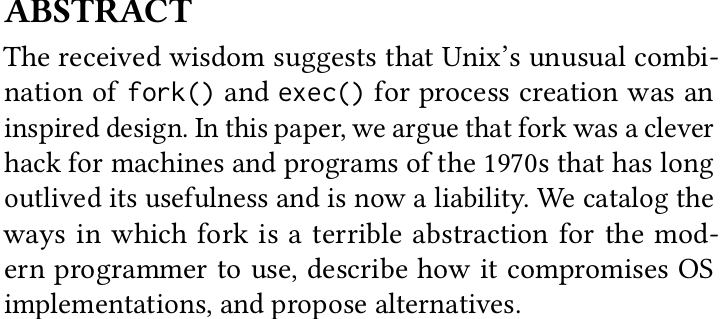
\includegraphics[width=5in]{../unix-api/fork-in-road-abs}
\end{frame}
